\section{Post Main Sequence}\label{sec:post-main-sequence}
Quando la stella finisce l'idrogeno all'interno del core si passa alla fase finale dell'evoluzione stellare, chiamata \textit{post-MS}. 

\subsection{Sub e Red Giant Branch}\label{sec:SGB-RGB}
In una prima parte della post main sequence il nucleo si contrae e la temperatura aumenta, assieme alla pressione, bruciando gli strati di idrogeno esterni al nucleo in una fase chiamata \textit{Herztsprung Gap} per stelle pesanti o \textit{SGB} per stelle più leggere. Nel frattempo, mentre il core, ora pieno di elio, continua a contrarsi aumentando di massa e aumentando la propria temperatura, l'envelope si espande raffreddandosi rendendola appunto una \textit{Gigante Rossa}. Nella figura~\ref{fig:evo} i punti 3, 4 e 5 del diagramma H-R rappresentano queste transizioni, osservando che, benché la temperatura decresca repentinamente, la luminosità della stella rimane pressoché costante. Dall'equazione~\ref{eq:stefan-boltzmann}, sappiamo infatti che:
\[
    L = 4\pi \sigma R^2 T^4
\]
Perciò la diminuzione di temperatura e il relativo aumento di volume si compensano perfettamente cosicché la luminosità del corpo ci appaia invariata.

Per stelle poco massive la diminuzione di temperatura implica l'avvicinamento alla traccia di Hayashi, per questo motivo la struttura stellare risponde aumentando il proprio raggio e conseguentemente la sua luminosità. Per stelle più pesanti, invece, la variazione di luminosità non è così netta. 
\subsection{Flash dell'Elio}\label{sec:flash-He e Horizontal Branch}

A questo punto nei corpi più leggeri, si arriva ad un punto limite, detto limite di degenerazione elettronica, superato questo il gas non può più essere considerato perfetto ed il nucleo entra in uno stato di degenerazione. L'aumento di temperatura non riesce a contrastare quello di densità, rendendo il gas sempre meno comprimibile e ritardando l'innesco dell'elio. Nei corpi più massivi la struttura è termoregolata, per cui l'aumento di temperatura è seguito dall'aumento di pressione e del volume della stella, in modo tale da bilanciare la pressione di radiazione. In queste strutture il collasso del core è notevolmente più facile, innescando le reazioni termonucleari per la fusione dell'elio non appena la temperatura raggiunge $T \sim \SI{e8}{K}$.

La differenza tra le due possibilità si osserva anche nel diagramma H-R della figura~\ref{fig:evo}, dove per le ultime l'attivazione della fusione ad elio (passaggio dal punto 5 al punto 6) è molto rapida e non comporta una variazione significativa della luminosità. Per le stelle più leggere, invece, l'accensione della fusione ad elio avviene in condizioni di semi-degenerazione e ritardata (di circa $\sim 10^6 \mbox{ yr}$) a causa dell'assenza di termoregolazione, motivo per cui l'aumento di temperatura non coincide con l'aumento di pressione. Si raggiunge, quindi, uno stato d'instabilità termonucleare fino a che $\rho_c$ non aumenta bruscamente, facendo implodere il core, rimuovendo la degenerazione e provocando un'esplosione, alla quale ci si riferisce con il termine \textit{Flash dell'Elio}. Questa comporta una rapida espansione del volume del nucleo e quindi della stella intera a causa di moti convettivi.
\begin{figure}
    \centering
    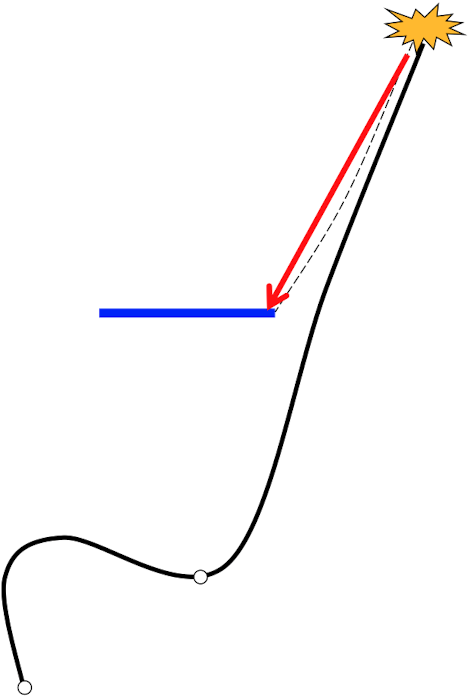
\includegraphics[width = 0.2\textwidth]{immagini/he_flash.png}
    \caption{La figura mostra la porzione del piano H-R in cui avviene il flash dell'elio assieme all'inizio dell' Horizontal branch.}\label{fig:flash-he}
\end{figure}

Dopo il flash dell'elio la produzione di energia diminuisce e così anche la luminosità della stella, fino a raggiungere la fase di \textit{Horizontal Branch} in cui questa rimane pressoché invariata. In questa parte della post-MS, raggiunta solo da stelle con massa inferiore alle $2.2 \si{\solarmass}$, non è presente degenerazione nel nucleo e si attiva la fusione di idrogeno negli strati più esterni della struttura, ancora pieni di idrogeno. Infatti, benché nel core l'idrogeno è stato consumato tutto durante la main sequence, negli strati più esterni, dove avveniva la trasmissione della radiazione, questo è ancora presente.

Nel piano H-R si osserva che l'esplosione dovuta all'accensione delle reazioni termonucleari ad elio avviene sempre quando la stella ha una massa intorno alle $0.5 \si{\solarmass}$ (nella figura~\ref{fig:evo} il punto 6 dell'evoluzione). Questo implica che la luminosità al momento del flesh dell'elio è uguale per tutte le stelle e che quindi tale fenomeno può essere utilizzato come indicatore di distanza dell'ammasso stellare, analizzando la magnitudine osservata e comparandola con quella assoluta.

Per stelle con una massa inferiore $M = 0.5\si{\solarmass}$ non è possibile attivare la reazione di fusione di elio nel core e per questo non sono in grado di attivare alcuna reazione termonucleare. Raggiungono quindi lo stato di \textit{Nana Bianca di elio (He Nana Bianca)}, una delle possibili morti stellari, in cui il nucleo rimane elettro degenere raffreddandosi lentamente, mentre gli strati più esterni rimangono liberi nella forma di nebulosa stellare.

Per quanto discusso nella sezione~\ref{sec:main-sequence}, una stella con massa inferiore a $M = 0.8 \si{\solarmass}$ passerà nella main sequence un periodo di tempo dell'ordine di grandezza dell'età del nostro universo. Inoltre, si è appena detto che le nane bianche si formano solo per stelle di massa inferiore a $M = 0.5 \si{\solarmass}$, questo vorrebbe dire che non è ancora possibile osservare questi tipi di corpi. Ciò nonostante questi corpi sono già presenti nei nostri cieli, com'è possibile? Quello che accade è che stelle nella fase SGB, con nuclei di elio, perdono i propri strati più esterni, per vari motivi (risucchio da parte di un'altra stella in sistemi binari, esplosione di una Supernova, ...).
\subsection{Asymptotic Giant Branch}\label{sec:asymptotic-giant-branch}

Si è arrivati al punto che le stelle con massa superiore a $M = 0.5 \si{\solarmass}$ sono in grado di riaccendere le reazioni termonucleari necessarie a fondere l'elio. Quando, però, finisce anche questo all'interno del core si arriva ad un bivio dettato ancora una volta dalla iniziale. 

Corpi con $M < 8\si{\solarmass}$ tornano in uno stato di nucleo degenere, ora composto da carbonio ed ossigeno, per cui non più in grado di attivare reazioni termonucleari, raggiungendo quello che viene chiamato il \textit{Ramo Asintottico delle Giganti (Asymptotic Giant Branch, AGB)}. La struttura di questa fase dell'evoluzione stellare è caratterizzata dall'attivazione della fusione negli strati più esterni, seguita poi dall'accensione della fusione dell'elio in quelli più interni (come mostrato in figura~\ref{fig:AGB}) in condizione di semi-degenerazione.
\begin{figure}
    \centering
    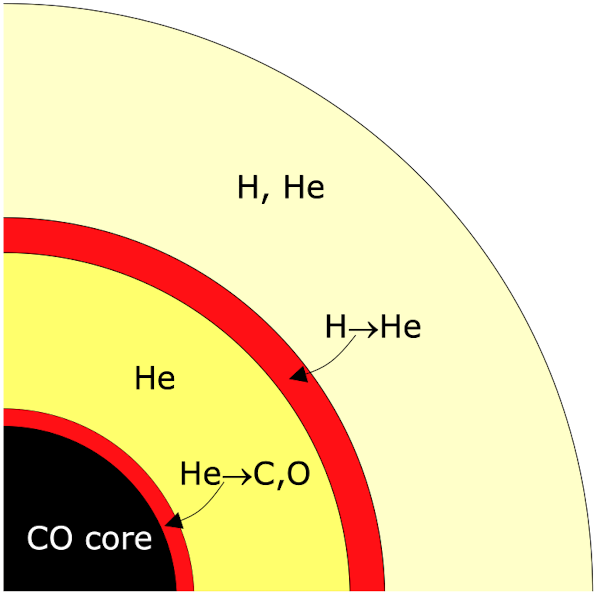
\includegraphics[width = 0.3 \textwidth]{immagini/AGB.png}
    \caption{La figura è una rappresentazione stilizzata della struttura stellare dopo la fine della fusione dell'Elio nel nucleo. Si osserva come negli strati dell'envelope si attivi la fusione di elementi progressivamente più leggeri allontanandosi dal centro della stella.}\label{fig:AGB}
\end{figure}
Quando anche l'elio si spegne, la stella si contrae e si attivano nuovamente le reazioni di fusione dell'idrogeno, osservando periodiche espansioni e contrazioni in un fenomeno chiamato \textit{Pulsazioni Termiche delle AGB (Thermal Pulse AGB)} dovute alla fusione periodica d'idrogeno ed elio. Nel piano H-R queste trasformazioni seguono la traccia di Hayashi parallelamente. Durante questi processi l'attrazione gravitazionale, per unità di superficie, sugli strati più esterni diminuisce a causa delle espansioni, comportando una perdita di materia rilasciandola nell'universo ad un rate di $\dot{M} \sim 10^{-4} \si{\solarmass} \mbox{ yr}^{-1}$. Si tratta di quasi una massa solare ogni $10000 \mbox{ yr}$, raggiungendo lo stato di \textit{Nebula planetaria} in cui non è più possibile attivare alcuna reazione termonucleare.

In questa ultima fase gli strati di elio ed idrogeno non sono abbastanza massivi da poter osservare alcuna attività termonucleare. La stella è definitivamente spenta. Il core si contrae aumentando la sua densità fino a raggiungere uno stato di degenerazione, mentre l'envelope si espande diventando un ammasso polveroso e di molecole fredde, rimanendo negli intorni di dove una volta era presente la stella. Quando la superficie di ciò che rimane raggiunge una temperatura di $T \sim \SI{e4}{K}$ parte dei gas e polveri presenti cominciano a ionizzarsi formando una nebulosa planetaria, che inizialmente non permette di osservare cosa resta del nucleo, a causa dell'elevata opacità. Queste strutture sono composte dagli elementi chimici generati dalle varie fusioni nucleari, in particolare elementi di tipo \textit{s}, carbonio, ossigeno, litio ed elementi pesanti dovuti al CNO.